\documentclass[10pt]{oblivoir}

% ---------------------------------------------- PACKAGE IMPORTS
\usepackage{kotex}
\usepackage{amsmath}
\usepackage{multicol}
\usepackage{fixltx2e}
\usepackage{float}
\usepackage{graphicx}
\usepackage{fullpage}
\usepackage{siunitx}
\usepackage[ruled,vlined]{algorithm2e}
\usepackage{hyperref}
\usepackage{listings}
\usepackage{color}
\usepackage{caption}
\usepackage{indentfirst}
\usepackage{subcaption}
\usepackage{tikz-cd}
\usepackage{chngcntr}
\usepackage{comment}
\usepackage[nameinlink]{cleveref}

% ---------------------------------------------- FIGURE COUNTER SETTINGS
% \counterwithin{figure}{section}

% ---------------------------------------------- CODE AREA SETTINGS
\definecolor{dkgreen}{rgb}{0,0.6,0}
\definecolor{gray}{rgb}{0.5,0.5,0.5}
\definecolor{mauve}{rgb}{0.58,0,0.82}

\lstset{frame=tb,
  language=C++,
  aboveskip=3mm,
  belowskip=3mm,
  showstringspaces=false,
  columns=flexible,
  basicstyle={\small\ttfamily},
  numbers=none,
  numberstyle=\tiny\color{gray},
  keywordstyle=\color{blue},
  commentstyle=\color{dkgreen},
  stringstyle=\color{mauve},
  breaklines=true,
  breakatwhitespace=true,
  tabsize=3
}

% ---------------------------------------------- CLEVERREF SETTINGS
\crefname{figure}{그림}{그림}
\crefname{equation}{식}{식}
\crefname{table}{표}{표}
\crefname{listing}{목록}{목록}
\crefname{section}{절}{절}
\crefname{algorithm}{알고리즘}{알고리즘}

\captionsetup[subfigure]{subrefformat=simple,labelformat=simple}
    \renewcommand\thesubfigure{ (\alph{subfigure})}

% ---------------------------------------------- GENERAL SETTINGS
\setlength{\parindent}{0.3cm} % The first indent width setup

% ---------------------------------------------- CUSTOM COMMANDS
%       GENERAL
\newcommand{\textss}[1]{\scriptsize#1\normalsize}
%       MATHEMATICAL
\newcommand{\abs}[1]{\left|\,#1\,\right|}

% ---------------------------------------------- HEADER
\title{AR 당구}
\author{강승우 \\ 한국기술교육대학교 전자공학과}
\date{2020.10}

% ---------------------------------------------- CONTENT
\begin{document}
\maketitle

\begin{figure}[ht]
    \centering
    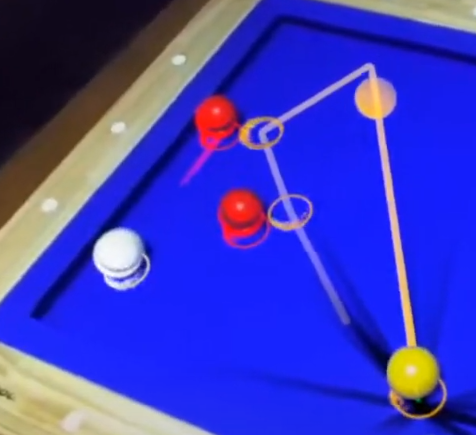
\includegraphics[width=5cm]{img/abstract-final.png}
\end{figure}

\begin{abstract}
    당구는 재미있는 스포츠이지만, 처음 입문한 초심자가 득점 가능한 경로를 계산하고 올바르게 공을 쳐서 보낼 정도로 숙련되기까지의 진입 장벽이 높은 편이다. 당구 초심자가 어느 정도 수준에 도달하기 위해선 지속적인 집중과 훈련을 필요로 하는데, 적절한 동기 부여 요소가 없다면 흥미를 잃어버리기 쉽다. 본 연구는 스테레오 카메라와 VR 카메라를 결합한 몰입도 높은 증강 현실 플랫폼 상에서 당구 경로 안내 및 시각 효과를 통해 초심자의 흥미를 유도하고 당구 학습을 가속하는 것을 목표로 두었다. 이를 위해 OpenCV를 활용하여 당구공 배치를 인식하고 Unity Engine 상에서 물리 시뮬레이션을 통해 경로 탐색과 시각화를 수행하였고, 그 결과 프로그램이 제안한 속도와 방향을 정확히 맞췄을 때 높은 정확도를 보였다. 이는 당구에 처음 입문하는 초심자가 경로 설계에 대한 부담 없이 공을 올바르게 보내는 훈련에만 집중할 수 있게 만들며, 나아가 오랜 시간 알고리즘이 제안하는 경로를 익힘으로써 점진적으로 당구 숙련도를 높일 수 있다는 점에서 AR 당구의 학습 보조 도구로서의 가능성을 확인할 수 있었다.
\end{abstract}

\newpage
\twocolumn[]

\begin{figure*}
    \centering
    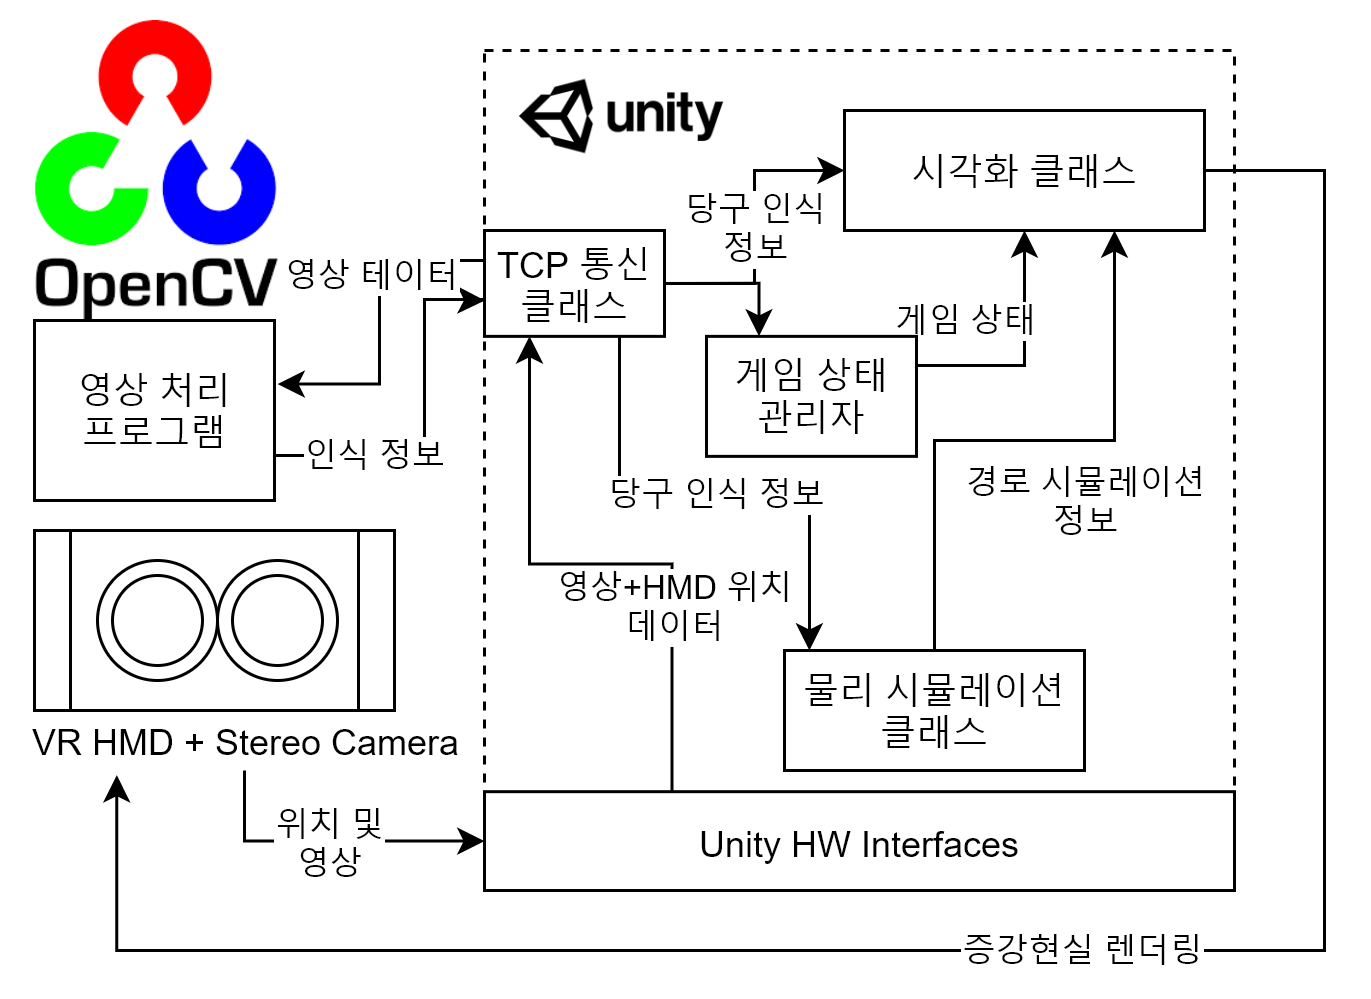
\includegraphics[width=14cm]{img/overall-process.png}
    \caption{시스템 구성}
    \label{fig;overall-proc}
\end{figure*}

\section{서론}
당구는 익숙해지기까지 많은 시간의 훈련과 적응을 필요로 하는 스포츠이다. 정보 매체의 발달로 학습을 필요로 하지 않는 직관적인 오락 컨텐츠가 폭발적으로 양산되는 시대에 이러한 진입 장벽은 초보자들이 발을 들이는 데 어려움으로 작용한다.

당구는 경로 설계와 큐잉(당구공을 큐로 치는 것) 두 가지가 모두 성공적으로 수행되었을 때 득점을 할 수 있다. 그러나 초보자가 나름대로 경로를 설계해 큐잉을 해도, 경로대로 공을 보내는 것 자체가 어려운 만큼 운이 아닌 실력만으로 득점을 내기는 쉽지 않다.

보통 당구는 체계적인 훈련이 아닌 놀이로서 시작하는 경우가 많으며, 놀이로서 학습을 지속하기 위해선 심리적인 보상이 필요하다. 당구에서는 득점이 이에 해당하는데, 상술한 진입 장벽에 빗대어 보면 당구 입문자는 실력이 갖춰질 때까지의 오랜 기간을 확실한 심리적인 보상 없이 훈련을 견뎌야 한다는 이야기가 된다.

% 무득점 = 동기 부여가 어려움
% 학습을 하다 지침

당구공의 경로 안내에 대한 아이디어는 바로 이러한 심리적인 보상 측면에서 출발한다. 아무런 보조 없이 당구를 연습하는 경우 초심자는 경로 설계와 큐잉 양단 모두를 병렬적으로 훈련해 나가야 하는데다 적절한 피드백을 받기도 어려우므로 학습을 지속하기가 어려웠다.

그러나 득점할 수 있는 경로를 알 수 있다면 초심자는 큐잉에만 온전하게 집중할 수 있으며, 어느 정도 큐잉에 익숙해진 후에는 시스템이 제공하는 경로 정보를 바탕으로 경로 설계에 대한 암시적인 경험을 쌓을 수 있다.

위의 아이디어를 바탕으로 이미 시중에는 당구대 상단에 카메라와 프로젝터를 설치하여 당구공의 배치를 분석해 경로를 안내하거나, 혹은 큐의 방향을 분석해 공의 진행 경로를 예측하는 프로젝트가 소개되었다.
\cite{AR-Pool-Projector} \cite{AR-Pool-Projector-2}

본 연구는 위 프로젝트와 맥락을 같이 하되, 주제의 구현에 점차 보편화되어가고 있는 증강 현실 장비를 활용한다. 이는 기존의 시스템에 비해 장소의 제약이 없는데다, 기존의 증강 현실 장비를 활용할 수 있으므로 적은 비용과 높은 범용성을 갖게 된다.


\section{제안 방식}
가상 현실 기술은 말 그대로 가상으로 세계를 만들고, 헤드 트래킹 기술을 통해 가상 세계의 카메라 위치를 사용자 눈의 위치와 동기화하여 사실적인 시청각 경험을 부여하는 기술이다.

가상 현실 어플리케이션은 기존의 전통적인 3D 게임에서 카메라의 제어만을 사용자가 장착한 HMD의 헤드 트래킹 신호에 위임한 것으로, 가상 현실 세계를 만드는 것은 3D 게임을 만드는 것과 다르지 않다.

이는 증강 현실 어플리케이션에서도 마찬가지이며, 따라서 실제 이미지 위에 증강 현실을 통해 이미지를 표시하기 위해선 먼저 영상 처리를 통해 실제 물체의 위치가 가상 현실 상에서 어느 좌표에 맵핑(mapping)되는지 파악할 필요가 있다.

본 연구에서는 카메라를 통해 입력된 이미지를 분석하여 당구대와 당구공의 카메라에 대한 상대 트랜스폼을 계산하고, 증강 현실 장비의 위치 추적 기능을 통해 얻은 가상 세계에서의 사용자의 머리 트랜스폼(카메라 위치 및 회전)를 활용해 이를 가상 세계의 절대 트랜스폼으로 변환한다.

당구대와 당구공의 위치가 파악되면 이를 바탕으로 물리 시뮬레이션을 수행할 수 있다. 이는 플레이어가 칠 공을 360도 전 방향에 대해, 다양한 속도로 타격 시뮬레이션을 수행한 뒤 득점하는 경로를 모두 파악하는 식으로 이루어진다.

시각화 기능은 사용자의 머리 위치 및 경로의 가중치에 따라 가장 합리적인 경로를 유니티 엔진의 다양한 파티클 시스템을 활용하여 시각화한다.

위의 세 과정은 별도의 트리거링 없이 시스템이 구동되는 내내 실시간으로 수행되며, 자세한 설계 방식은 아래에서 다룬다.

\subsection{영상 처리}
% 영상 인식 블록도
\begin{figure*}
    \centering
    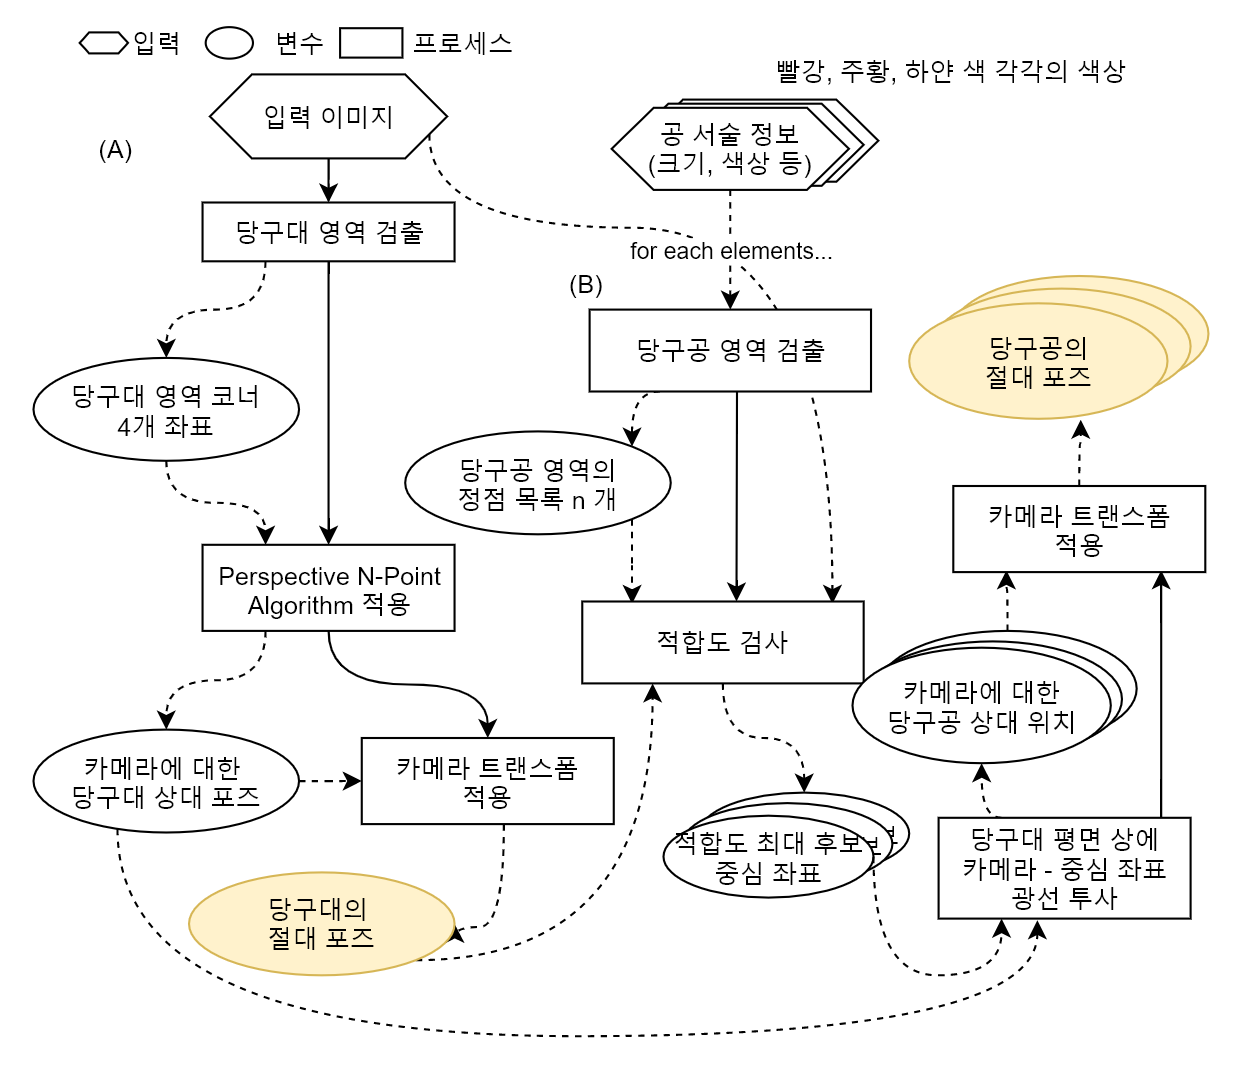
\includegraphics[width=16cm]{img/recognition-diagram.png}
    \caption{영상 인식 과정 요약}
    \label{fig;recognition-flowchart}
\end{figure*}

본 연구에 사용된 당구대의 펠트는 이미지 상에서 다른 물체와 뚜렷하게 구별되는 색상이다(\cref{fig;table}). 이를 HSV 색공간; 색상(Hue), 포화(Saturation, 색의 진한 정도), 명도(Value)로 변환하여 평가하면 균일한 색상을 갖는 당구대의 펠트 표면은 안정적인 색상과 포화 값을 갖게 된다.

\cref{fig;table-hsv-coloronly}는 이를 잘 나타내는데, 이는 HSV 색공간으로 변환한 이미지에서 명도 값을 255로 통일한 것으로 밝기의 영향을 없애자 당구대의 펠트 영역이 훨씬 더 선명하게 부각되고, 더불어 공의 색상도 뚜렷하게 구별되는 것을 알 수 있다.

\begin{figure}[ht]
    \centering
    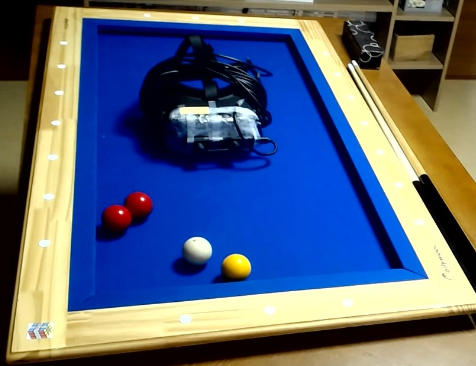
\includegraphics[width=7cm]{img/billiards-table.png}
    \caption{하드웨어 및 당구대 이미지}
    \label{fig;table}
\end{figure}

\begin{figure}[ht]
    \centering
    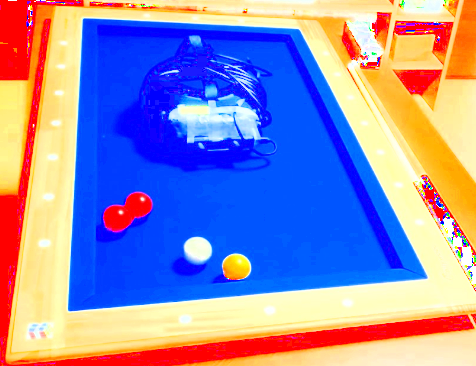
\includegraphics[width=7cm]{img/table-coloronly.png}
    \caption{명도를 제외하여 평가}
    \label{fig;table-hsv-coloronly}
\end{figure}

\cref{fig;table-hsv-coloronly}에서 테이블 영역의 색상과 포화 값은 뚜렷하게 구별되는 범위 내에 존재하므로, 단순히 H, S 값이 일정 범위 내에 있는 픽셀을 모두 골라내는 것만으로도 꽤 정확하게 당구대의 영역을 찾아낼 수 있다. 여기서는 OpenCV 라이브러리의 함수인 inRange()를 사용하며, 색상 값 165~15\si{\degree}이고 포화 값이 150~255 사이인 모든 픽셀을 True로 지정한다.

\begin{figure}[ht]
    \centering
    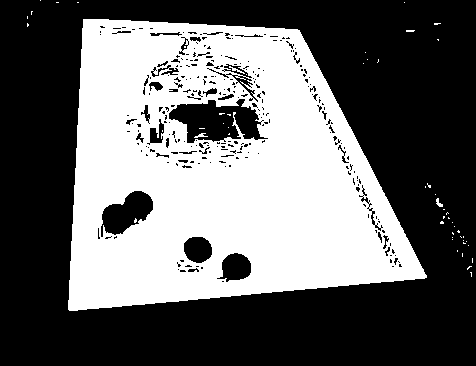
\includegraphics[width=0.4\textwidth]{img/billiards-table-filter.png}
    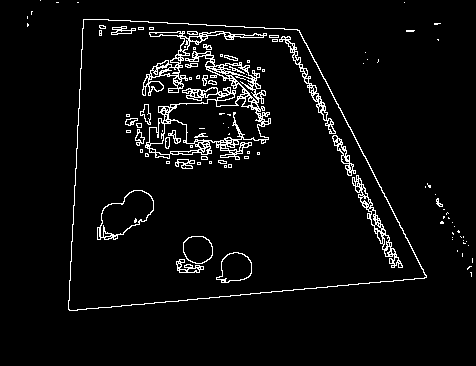
\includegraphics[width=0.4\textwidth]{img/billiards-table-edge.png}
    \caption{색상 및 포화에 대한 단순 필터링 및 경계 검출}
    \label{fig;table-filtered}
\end{figure}

필터링 결과인 이진 이미지 \cref{fig;table-filtered}로부터, OpenCV의 findContours() 함수를 통해 이미지 내에 존재하는 모든 도형을 찾아낼 수 있다. 각 도형은 해당 도형을 이루는 꼭지점의 좌표 목록으로 구성되어 있다.

그러나 findContours() 함수의 알고리즘은 직선 여부를 엄격하게 평가하기 때문에 \cref{fig;table-filtered}의 사각형 도형은 네 개보다 훨씬 많은 수의 정점(\cref{fig;table-many-dots})으로 평가된다. 따라서 OpenCV의 approxPolyDP() 함수에 $\epsilon = 5$ (\textit{Ramer Douglas Peucker algorithm})를 지정하여 다수의 정점을 일정 범위 내에서 직선으로 근사한다.

이후 당구 큐대 등 다른 오브젝트에 의해 당구대 영역이 침범당하는 경우 등에도 당구대의 꼭지점 네 개가 화면 안에 있는 한 당구대 영역이 검출될 수 있게끔 OpenCV의 convexHull() 함수를 적용해 모든 당구대 영역을 볼록 다각형으로 만들어준다.

\begin{figure}[ht]
    \centering
    \begin{subfigure}{0.4\textwidth}
        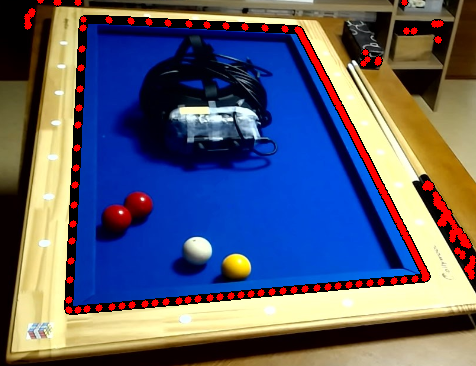
\includegraphics[width=\textwidth]{img/billiards-table-contours-dot-view.png}
        \caption{직선 근사 전}
        \label{fig;table-many-dots}
    \end{subfigure}
    \begin{subfigure}{0.4\textwidth}
        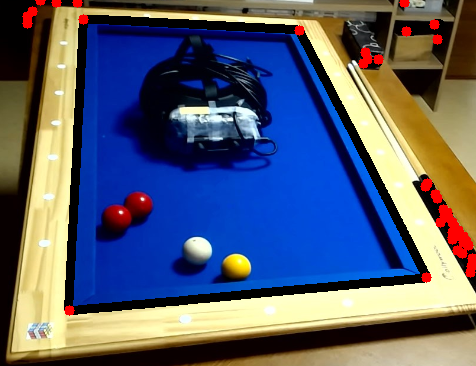
\includegraphics[width=\textwidth]{img/billiards-table-contours-dot-view-approx.png}
        \caption{직선 근사 후}
        \label{fig;table-approximated}
    \end{subfigure}
    \caption{}
\end{figure}

이를 통해 이미지 상에서 당구대와 같은 색상을 갖는 모든 영역에 대한 도형 정점 집합을 획득하게 된다. 이 때 당구대의 꼭지점 개수가 4개인 것은 자명하고, 사용자가 당구대를 바라보고 있다면 당구대 영역의 크기 또한 화면 상에서 일정 이상을 차지할 것이다.

따라서 각각의 도형을 반복하여 조건에 부합하는 도형을 찾고, 이를 당구대의 네 개 꼭지점이라 가정한다. 여기까지의 과정이 \cref{fig;recognition-flowchart}의 당구대 영역 검출에 해당한다(\cref{fig;table-approximated}).

당구대는 변형되지 않는 강체(rigid body)이며, 당구대의 치수는 이미 알고 있다. \cref{fig;table-on-origin}과 같이, 당구대와 치수가 같은 물체가 원점(0, 0, 0)에 있다고 가정한다. 카메라 또한 원점에서 정면(z축)을 바라보고 있다면, 테이블의 $\frac{1}{4}$정도만이 카메라의 시야에 들어올 것이다.

\begin{figure}
    \centering
    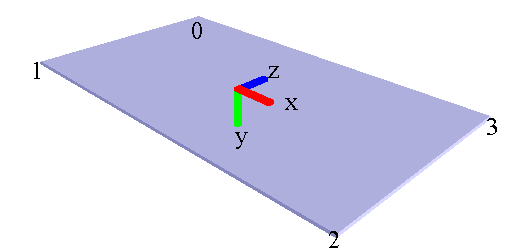
\includegraphics[width=0.4\textwidth]{img/table-3d.pdf}
    \caption{원점에 위치한 당구대}
    \label{fig;table-on-origin}
\end{figure}

\cref{fig;table-on-origin}를 옮기면 카메라에 보이는 당구대의 모양이 원근법에 따라 바뀔 것이며, 당구대와 같은 치수를 가지므로 특정 위치와 회전에서 당구대 치수의 물체가 실제 당구대의 영역을 정확하게 덮게 된다. 이 때의 특정 위치와 회전가 물체의 포즈(pose)이다.

기술적으로는 화면 상에서 검출된 4개의 2차원 점과 원점에 있는 물체의 4개의 3차원 점이 각각 목적지와 모델을 나타내며, 여러 가지 트랜스폼에 대해 원점의 4개 정점을 변환하고 카메라 화면 상에 투영하여 목적지의 4개 점과 수렴할 때까지 반복한다.

위의 절차는 \textit{Perspective N Point Algorithm}으로, \\OpenCV의 solvePnP() 함수로 구현된다. 단, 함수 내부적으로는 포즈를 계산할 정점 집합의 순서가 정합되었다고 가정하므로, 화면 상에 검출된 정점의 목록도 짧은 변을 이루는 인덱스가 먼저 나타나도록 순서를 조정해주어야 한다. 이는 스테레오 카메라로부터 얻은 깊이 맵을 활용한다.

\begin{figure}
    \centering
    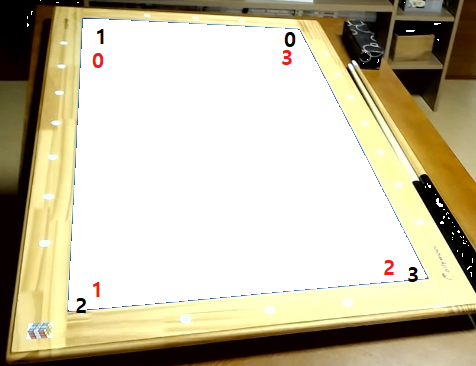
\includegraphics[width=0.4\textwidth]{img/billiards-table-indexes.png}
    \caption{인덱스 정합의 예시}
\end{figure}

PNP 알고리즘을 적용하면 상대 포즈 $\textbf{T}_{r}$; 카메라에 대한 당구대의 위치 및 회전 정보를 얻을 수 있다.

당구대 평면의 위치를 알고 있고, 또 당구공의 중점은 반드시 당구대 평면(여기서는 당구대 바깥쪽 쿠션의 포즈를 구했으므로)상에 위치하므로 이미지 상에서 당구공의 중점을 계산하여, 카메라 원점에서 당구공 중점 방향으로 광선을 투사해 당구대 평면과 부딪치는 점을 찾으면 그것이 당구공의 중점이 된다.

이를 통해 위에서 내려다보는 형태의 시점이 아니라도 정확하게 당구공의 중점을 계산할 수 있다.

\begin{figure}
    \centering
    \begin{subfigure}{0.4\textwidth}
        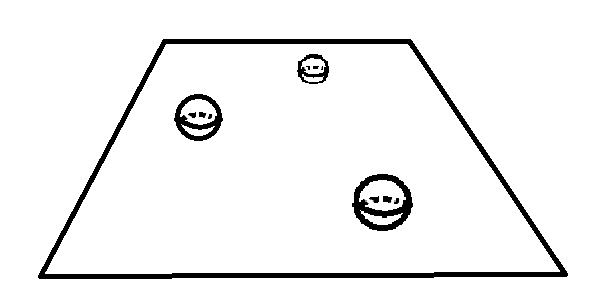
\includegraphics[width = \textwidth]{img/ball-recognition-introduce.png}
        \caption{당구공의 중심은 반드시 한 평면상에 존재}
    \end{subfigure}
    \begin{subfigure}{0.4\textwidth}
        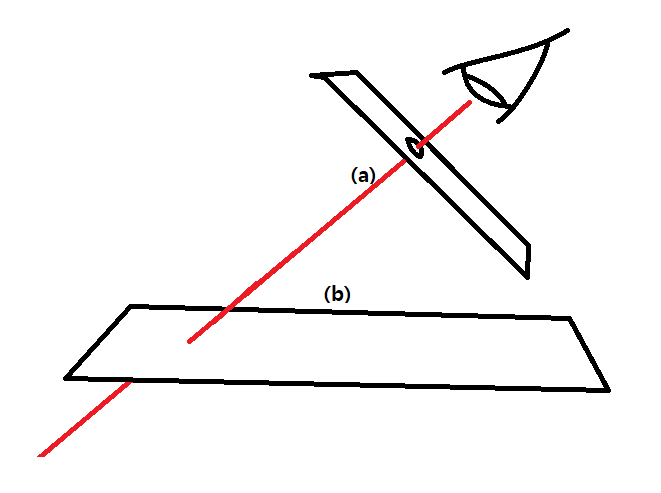
\includegraphics[width=\textwidth]{img/ball-recognition-howto.png}
        \caption{당구공의 중점 방향으로 광선 투사}
        \label{fig;raycast-to-table}
    \end{subfigure}
    \caption{}
\end{figure}

이를 위해 먼저 당구공의 중점의 위치를 찾아야 한다. \cref{fig;table-hsv-coloronly}에서 볼 수 있듯 각 공은 색상 및 포화 영역에서 매우 뚜렷하게 구별된다. 또한, \cref{fig;table-filtered}의 경계선 이미지에서 외부의 테이블 영역과, 음영으로 인해 생긴 작은 잡음들을 제거한 후 앞서 언급한 함수 findContours를 적용하면, 테이블의 영역이 아닌 곳, 즉 공이 위치할 가능성이 있는 모든 영역의 등고선을 얻을 수 있다.

각 등고선을 반복하여 등고선의 정점 목록을 감싸는 사각형 영역으로 관심 영역을 지정, 당구공이 존재할 가능성이 있는 높은 영역에만 중심 후보를 두고 연산을 적용해 최적화를 수행한다.

각 관심 영역 내에서, 공을 찾기 위해 일종의 변형된 템플릿 매칭을 적용한다.

먼저 전체 HSV 이미지에서 각 공의 색상에 해당하는 HSV 중간값의 각 채널을 단순히 빼고, 각 채널에 가중치($k_h, k_s, k_v$)를 두어 해당 픽셀과 레퍼런스 색상 $h_0$, $s_0$, $v_0$ 사이의 유클리드 거리 $d_n$을 계산한다. $d_n$에 오차의 영향을 제어하는 상수 $k_e$를 곱한 값의 음수를 지수함수로 계산하면, 오차가 없는 경우 1, 오차가 클수록 0에 수렴하는 형태의 적합도 값 $s_n$을 얻을 수 있다.

이 과정을 식으로 나타내면 다음과 같다.
$$ d_{n} = \sqrt{k_h(h_0-h_n)^2+k_s(s_0-s_n)^2+k_v(v_0-v_n)^2} $$
$$ s_{n} = e^{-d_{n}k_{e}} $$

본 연구에서 픽셀의 각 채널 오차에 대한 가중치 $k_h$, $k_s$, $k_v$는 각각 2, 1, 0을 지정하였다. 이는 즉 명도의 오차는 고려하지 않으며, 포화도의 오차보다 색상의 오차의 영향을 더 높게 친다는 의미이다.

또한 빨간색, 주황색, 흰색 각각은 색상, 포화도 값을 $(130, 160)$, $(90, 180)$, $(40, 50)$로 두고 가중치를 계산한다(명도는 고려하지 않았다). 단, 이는 8비트 범위인 0\~{}255 사이의 값이므로 위 식에서 $h_0$, $s_0$으로 사용될 때는 $255.0$으로 나누어 0\~{}1로 정규화한다.

위 과정을 모든 픽셀에 대해 적용하면 각 색상별로 적합도 맵을 얻을 수 있으며, 각각의 점에 대해 화면 상에 보이는 공의 반지름 크기의 커널로 콘볼루션 연산을 적용, 가장 높은 값을 반환하는 픽셀을 당구공의 중점으로 결정한다.

그러나 \cref{fig;table-hsv-coloronly}에서 볼 수 있듯 카메라에 가까운 부분과 먼 부분의 공 크기가 서로 달라 고정된 크기의 커널을 전체 이미지에 적용하면 정확한 결과를 얻을 수 없다. 따라서 추정 중점으로 투사한 광선과 테이블의 접점으로부터 해당 점과 카메라 사이의 거리를 계산하고, 이로부터 당구공의 추정 반지름을 계산해 더 알맞는 커널을 적용, 적합도의 합을 계산한다.

이렇게 계산된 당구공의 중점 방향으로, 카메라 위치가 원점인 광선을 투사해 당구대와 충돌하는 점이 카메라에 대한 당구공의 상대 위치가 된다(\cref{fig;raycast-to-table}).

당구대와 당구공의 상대 위치에 AR 헤드셋의 위치 추적 기능이 보고한 카메라 트랜스폼을 적용하면, 당구대와 당구공의 AR 공간에서의 절대 좌표를 획득할 수 있다. 이것이 \cref{fig;overall-proc}의 영상 처리 프로그램이 Unity 어플리케이션으로 전송하는 인식 정보에 해당한다.

\subsection{물리 시뮬레이션}
당구대와 네 공의 절대 위치를 모두 아는 경우, 물리 시뮬레이션을 통해 플레이어가 친 공의 경로를 시뮬레이션하고 득점이 나는 경우를 계산해낼 수 있다.

일반적으로 물리 시뮬레이션은 시분할, 또는 타임 스텝이라 불리는 이산적인 방법에 의해 제어된다. 예를 들어 시점 $n$에서 물체의 가속도가 $\vec{a}_n$이고, 시뮬레이션 간격이 $\delta{t}$일 때 각각의 시뮬레이션 단계에서 다음 속도와 위치를 다음과 같이 계산하는 식이다.

$$ \vec{v}_{n+1} = \vec{v}_n + \vec{a}_n\delta{t} $$
$$ \vec{s}_{n+1} = \vec{s}_n + \vec{v}\delta{t} $$

이는 적분 연산을 단순화하므로 복잡한 물리 수식과 점화식의 도입이 자유롭다는 장점이 있다. 또한 시뮬레이션 간격 $\delta{t}$를 조절함으로써 시뮬레이션의 정확도와 최적화 수준을 제어할 수 있다.

그러나 시분할 방식의 시뮬레이션은 전체 시뮬레이션의 길이, 그리고 정확도 수준에 따라 연산량이 선형적으로 증가한다. 이는 경로 탐색을 위해 공의 타격을 360도 방향으로, 다양한 속도에 걸쳐 수천 회 이상 시뮬레이션 해야 하는 AR 당구의 환경에서는 큰 단점으로 작용한다. 

따라서 본 연구에선 시분할이 아닌 이벤트 기반의 물리 시뮬레이션 기능을 설계한다. 시뮬레이션은 당구공과 쿠션의 물리만을 고려한 단순한 구 및 평면 모델만을 사용한다. 

일반적인 시분할 시뮬레이션이 \cref{algo;timestep}과 같이 고정된 시간 간격에 대해 업데이트를 수행하고 충돌 여부를 검사하는 것과 달리, 이벤트 기반 시뮬레이션은 \cref{algo;event-driven}에서와 같이 전체 시뮬레이션 길이에 대해 충돌 검사를 모두 수행한 후, 가장 먼저 충돌이 발생하는 시간을 선택해 해당 시간만큼만 시간을 진행시킨 뒤 충돌 처리를 수행, 이를 반복하는 방식으로 구현된다.

\begin{algorithm}
    \caption{일반적인 시분할 시뮬레이션}
    \label{algo;timestep}
    input colliders : set of collision objects\\
    input duration : total simulation duration \\
    input delta : fixed delta time step \\
    output collisions : list of all collisions \\
    \While{duration > 0}{
        \ForEach{collider in colliders}{
            \CommentSty{// advances movement} \\
            collider.updateAcceleration(delta) \\
            collider.updateVelocity(delta) \\
            collider.updatePosition(delta) 
        }
        
        \ForEach{A in colliders}{
            B = next iterator of A \\
            \While{B is in colliders}{
                collisionResult = A.calculateCollision(B) \\
                \If(){collisionResult exists}{
                    collisions.add(collisionResult)
                }
                B = next iterator of B
            }
        }
        
        duration = duration - delta
    }
\end{algorithm}

\begin{algorithm}
    \caption{이벤트 기반 시뮬레이션}
    \label{algo;event-driven}
    input colliders : set of collision objects\\
    input duration : total simulation duration \\
    output collisions : list of all collisions \\
    \While{duration > 0}{
        minimumTime = duration \\
        fastestCollision = empty \\
        \ForEach{A in colliders}{
            B = next iterator of A \\
            \While{B is in colliders}{
                collisionResult = A.calculateCollision(B, duration) \\
                \If(){collisionResult.time < minimumTime}{
                    minimumTime = collisionResult.time \\
                    fastestCollision = collisionResult
                }
                B = next iterator of B
            }
        }
        
        \ForEach{collider in colliders}{
            collider.advanceMovement(minimumTime)
        }
        
        \If(){fastestCollision exists}{
            A = fastestCollision.A
            B = fastestCollision.B
            A.applyCollision(B)
            collisions.add(fastestCollision)
        }
        
        duration = duration - minimumTime
    }
\end{algorithm}

이 방법을 사용하면 O($n^2$)의 높은 복잡도를 가진 충돌 검사 연산을 시분할 방식에 비해 극적으로 적게 수행할 수 있다. 이때 충돌 검사는 구체 궤적 교차(swept sphere intersection) 검사 및, 일반적인 점 궤적-평면 간 교차 검사를 통해 수행한다. \cite{GameProgramming:Sanjay}



% 물리 시뮬레이션 설계 방식

% 시각화 방식

\section{실험 결과}
% 테이블 필터링 과정

% 공 인식 과정

% 물리 시뮬레이션 설계 영상

\section{결론}

\bibliographystyle{ieeetr}
\bibliography{content.bib}

\end{document}
